\documentclass[a4paper,11pt]{article}
\usepackage{amsmath,amsthm,amsfonts,amssymb,amscd,amstext,vmargin,graphics,graphicx,tabularx,multicol} \usepackage[french]{babel}
\usepackage[utf8]{inputenc}  
\usepackage[T1]{fontenc} 
\usepackage[T1]{fontenc}
\usepackage{amsmath,amssymb}
\usepackage{pstricks-add,tikz,tkz-tab,variations}
\usepackage[autolanguage,np]{numprint} 
\usepackage{color}
\usepackage{ulem}
\usepackage{mathrsfs}  

\setmarginsrb{1.5cm}{0.5cm}{1cm}{0.5cm}{0cm}{0cm}{0cm}{0cm} %Gauche, haut, droite, haut
\newcounter{numexo}
\newcommand{\exo}[1]{\stepcounter{numexo}\noindent{\bf Exercice~\thenumexo} : \marginpar{\hfill /#1}}
\reversemarginpar


\newcounter{enumtabi}
\newcounter{enumtaba}
\newcommand{\q}{\stepcounter{enumtabi} \theenumtabi.  }
\newcommand{\qa}{\stepcounter{enumtaba} (\alph{enumtaba}) }
\newcommand{\initq}{\setcounter{enumtabi}{0}}
\newcommand{\initqa}{\setcounter{enumtaba}{0}}

\newcommand{\be}{\begin{enumerate}}
\newcommand{\ee}{\end{enumerate}}
\newcommand{\bi}{\begin{itemize}}
\newcommand{\ei}{\end{itemize}}
\newcommand{\bp}{\begin{pspicture*}}
\newcommand{\ep}{\end{pspicture*}}
\newcommand{\bt}{\begin{tabular}}
\newcommand{\et}{\end{tabular}}
\renewcommand{\tabularxcolumn}[1]{>{\centering}m{#1}} %(colonne m{} centrée, au lieu de p par défault) 
\newcommand{\tnl}{\tabularnewline}

\newcommand{\trait}{\noindent \rule{\linewidth}{0.2mm}}
\newcommand{\hs}[1]{\hspace{#1}}
\newcommand{\vs}[1]{\vspace{#1}}

\newcommand{\N}{\mathbb{N}}
\newcommand{\Z}{\mathbb{Z}}
\newcommand{\R}{\mathbb{R}}
\newcommand{\C}{\mathbb{C}}
\newcommand{\Dcal}{\mathcal{D}}
\newcommand{\Ccal}{\mathcal{C}}
\newcommand{\mc}{\mathcal}

\newcommand{\vect}[1]{\overrightarrow{#1}}
\newcommand{\ds}{\displaystyle}
\newcommand{\eq}{\quad \Leftrightarrow \quad}
\newcommand{\vecti}{\vec{\imath}}
\newcommand{\vectj}{\vec{\jmath}}
\newcommand{\Oij}{(O;\vec{\imath}, \vec{\jmath})}
\newcommand{\OIJ}{(O;I,J)}

\newcommand{\bmul}[1]{\begin{multicols}{#1}}
\newcommand{\emul}{\end{multicols}}


\newcommand{\reponse}[1][1]{%
\multido{}{#1}{\makebox[\linewidth]{\rule[0pt]{0pt}{20pt}\dotfill}
}}

\newcommand{\titre}[5] 
% #1: titre #2: haut gauche #3: bas gauche #4: haut droite #5: bas droite
{
\noindent #2 \hfill #4 \\
#3 \hfill #5

\vspace{-1.6cm}

\begin{center}\rule{6cm}{0.5mm}\end{center}
\vspace{0.2cm}
\begin{center}{\large{\textbf{#1}}}\end{center}
\begin{center}\rule{6cm}{0.5mm}\end{center}
}



\begin{document}
\pagestyle{empty}


\begin{center}
\begin{Large}
\textbf{Calculs de volumes}
\end{Large}

\end{center}

\vspace*{1cm}

\exo{} Tous ces solides ont la même hauteur : h = 4 cm. Après avoir calculer le volume de chacun d'eux, citer le solide qui a le volume le plus grand.
\begin{flushleft}
\includegraphics[scale=0.85]{volume1.eps} 
\end{flushleft}

\color{red}

Dans un premier, on va calculer le volume de chaque solide.\\
Je rappelle la formule qui est la même pour une pyramide ou un cône de révolution :\\

$ V = \dfrac{\mathscr{B}  \times h}{3}$\\

\bmul{3}
\textbf{Le cône de révolution :}\\

$A_{disque}= \pi \times r^{2}$\\
$A_{disque}\approx 3,14 \times 3^{2}$\\
$A_{disque}\approx 28,26 cm^{2}$\\

$ V_{cone} = \dfrac{\mathscr{B}  \times h}{3}$\\
$ V_{cone} \approx \dfrac{28,26  \times 4}{3}$\\
$ V_{cone}\approx 37,68 cm^{3}$\\

\columnbreak

\textbf{La pyramide ABCDE :}\\

$A_{rectangle}= L \times l$\\
$A_{rectangle}=8 \times 1$\\
$A_{rectangle}=8 cm^{2}$\\

$ V_{ABCDE} = \dfrac{\mathscr{B}  \times h}{3}$\\
$ V_{ABCDE} = \dfrac{8  \times 4}{3}$\\
$ V_{ABCDE} \approx 10,67 cm^{3}$\\

\columnbreak

\textbf{La pyramide RDITV :}\\

$A_{rectangle}= L \times l$\\
$A_{rectangle}=3 \times 2,5$\\
$A_{rectangle}=7,5 cm^{2}$\\

$ V_{RDITV} = \dfrac{\mathscr{B}  \times h}{3}$\\
$ V_{RDITV} = \dfrac{7,5 \times 4}{3}$\\
$ V_{RDITV} = 10 cm^{3}$\\

\emul


\textbf{La pyramide SABC :}\\

$A_{triangle}= \dfrac{b \times h}{2}$\\
$A_{triangle}=\dfrac{3 \times 5,1}{2}$\\
$A_{triangle}=7,65 cm^{2}$\\

$ V_{SABC} = \dfrac{\mathscr{B}  \times h}{3}$\\
$ V_{SABC} = \dfrac{7,65 \times 4}{3}$\\
$ V_{SABC} = 10,2 cm^{3}$\\





\fbox{$V_{RDITV}<V_{SABC}<V_{ABCDE}<V_{cone}$} \\

 Le solide avec le plus grand volume est \textbf{le cône de révolution}.\\

\end{document}
